\documentclass{article}

\usepackage{parskip}
\usepackage{fullpage}
\usepackage{booktabs}
\usepackage{tikz}
\pagenumbering{gobble}

\begin{document}

Roll two ten sided dice 10 times to obtain the coordinates of ten points.
Record the coordinates in the following table:

    \begin{center}
        \begin{tabular}{lcc}
            \toprule
            Point&$x$&$y$\\
            \midrule
            1&&\\
            2&&\\
            3&&\\
            4&&\\
            5&&\\
            6&&\\
            7&&\\
            8&&\\
            9&&\\
            10&&\\
            \bottomrule
        \end{tabular}
    \end{center}

\rule{\textwidth}{.2pt}

Draw the points on the following grid:\\

    \begin{center}
        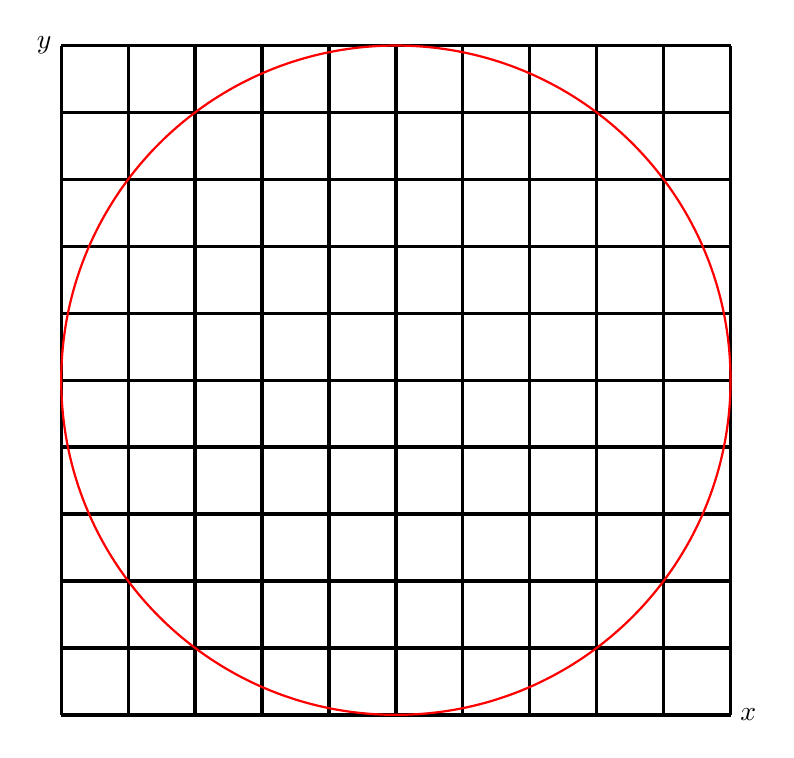
\begin{tikzpicture}[scale=.85]
        \draw[step=1cm,black,very thick] (0,0) grid (10,10);
        \draw [thick, red](5,5) circle (5cm);
        \node at (0,10) [left] {$y$};
        \node at (10,0) [right] {$x$};
        \end{tikzpicture}
    \end{center}

\rule{\textwidth}{.2pt}

Count the number $n$ of points that lie within the {\color{red}{red}} circle:

    $$n = $$

Calculate:

    $$4\frac{n}{N}=$$

where $N=10$ is the number of points in total.

\end{document}
